\documentclass{beamer}
\usepackage[utf8]{inputenc}
\usepackage{amssymb}
\usepackage{xcolor}

\title[Nelder-Mead on the Rheology Problem]{Chapter 5 Project: Apply Nelder-Mead to the Rheology Problem}
\author[Matthew, Tyler, and Sarah]{Matthew Saurette, Tyler ``can put his hand in his mouth" Weames, and Sarah Wyse}
\institute[Math 462]{Math 462\\ University of British Columbia - Okanagan}
\date{December 2020}
\usetheme{Madrid}
\usecolortheme{seahorse} 
\useinnertheme{rounded}

\begin{document}
\maketitle


%%%%The Rheology Problem
%------------------------------------------------------------------------
\begin{frame}{The Rheology Problem}
\begin{block}{Viscosity of a system}
$$\eta(\dot{\gamma}) = \eta_0(1+\lambda^2\dot{\gamma}^2)^{\frac{\beta -1}{2}}$$
A function of the strain rate, $\dot{\gamma}$, with parameters $\eta_0$, $\lambda$, and $\beta$.
\end{block}
\begin{columns}
	\begin{column}{0.45\linewidth}
		\centering
		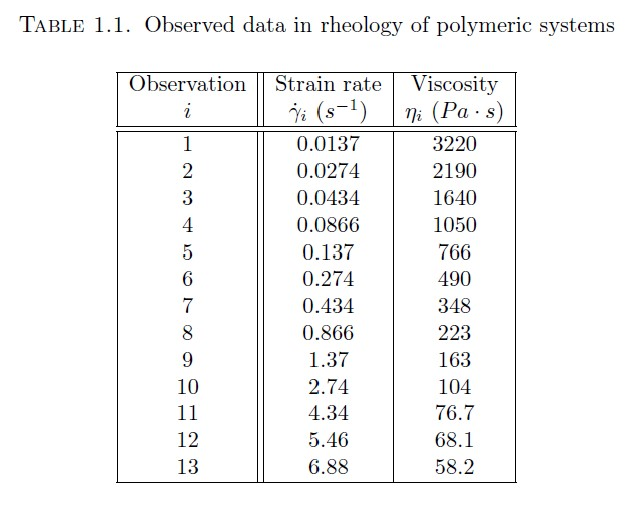
\includegraphics[width=0.95\linewidth]{Data}
	\end{column}
	\begin{column}{0.53\linewidth}
		Absolute Error:
		$$\epsilon_i(\eta_0, \lambda, \beta) = |\eta_0(1+\lambda^2\dot{\gamma}^2)^{\frac{\beta -1}{2}} - \eta_i|$$
		Non-smooth optimization problem:
		$$\hat{g}(\eta_0, \lambda, \beta) = \sum\limits_{i=1}^{13}\epsilon_i(\eta_0, \lambda, \beta)$$
	\end{column}
\end{columns}
\hfill \tiny (Audet and Hare, 2017)
\end{frame}

%%%%The NM Algorithm
%-------------------------------------------------------------------------
\begin{frame}{Nelder-Mead Algorithm}
    \centering
    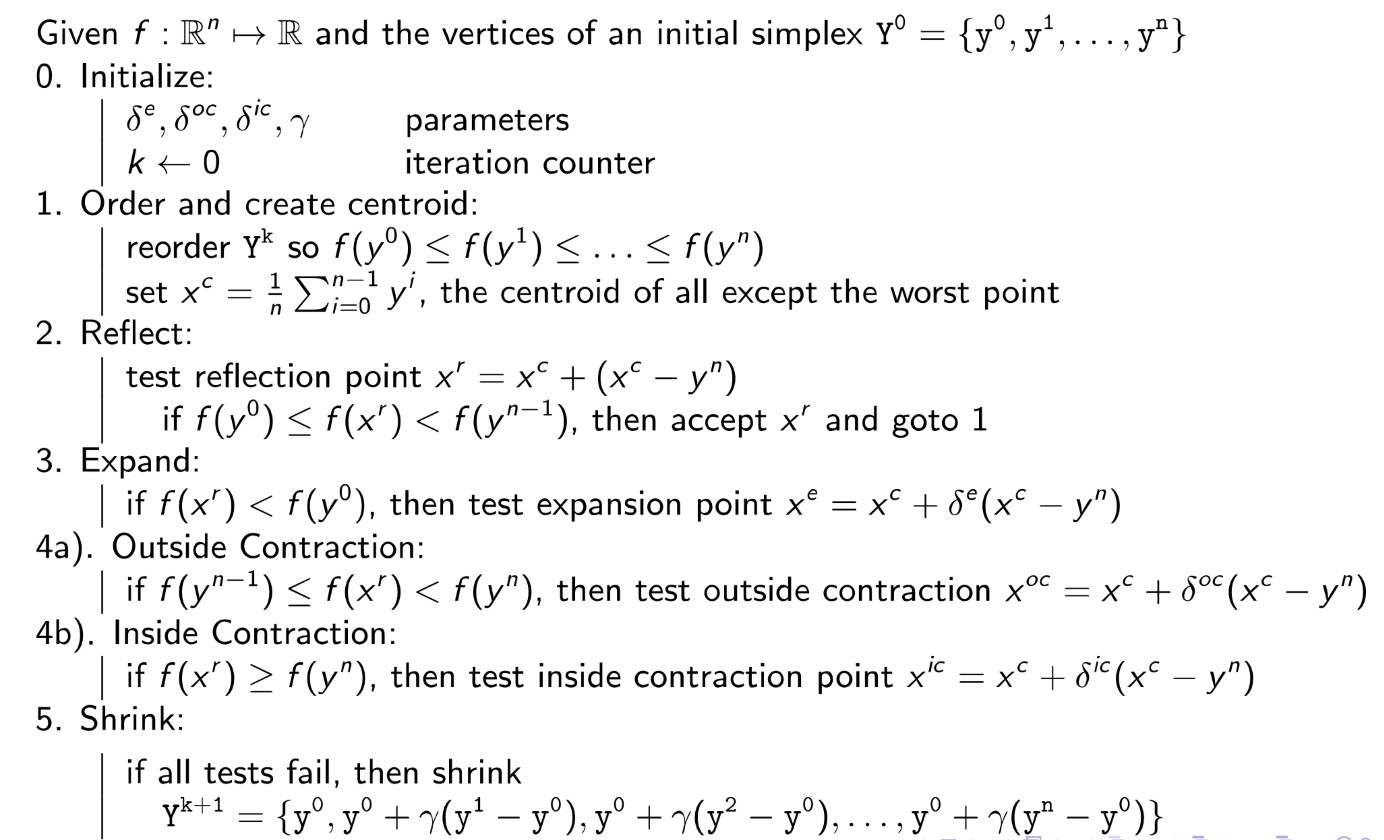
\includegraphics[width=0.95\linewidth]{NMAlgorithm}\\
	\hfill \tiny (Math 462, UBCO, 2020) 
\end{frame}

\begin{frame}{0. Initialize}
	\centering
	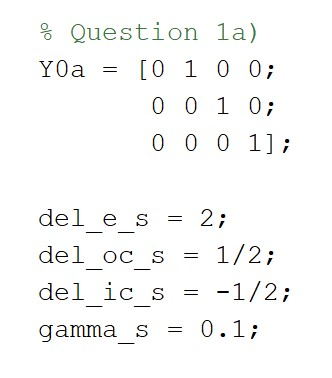
\includegraphics[width=0.35\linewidth]{Initialize}
	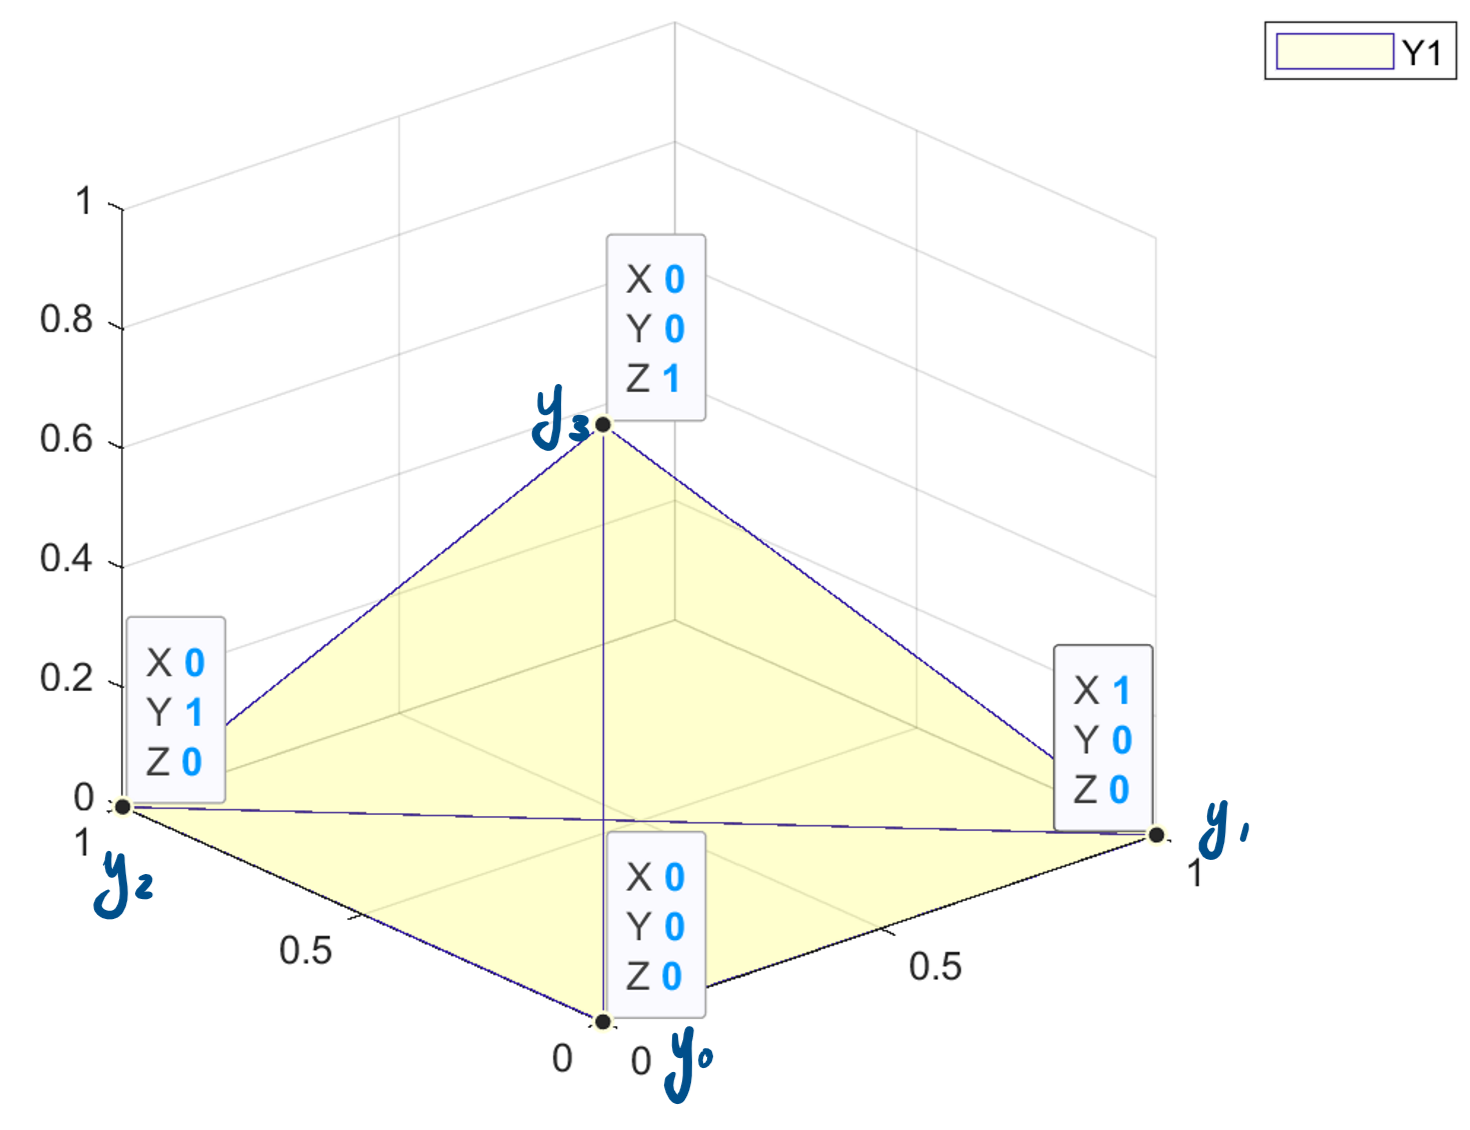
\includegraphics[width=0.59\linewidth]{InitializeFig}
\end{frame}

\begin{frame}{1. Order}
	\begin{columns}
	\begin{column}{0.35\linewidth}
		\centering
		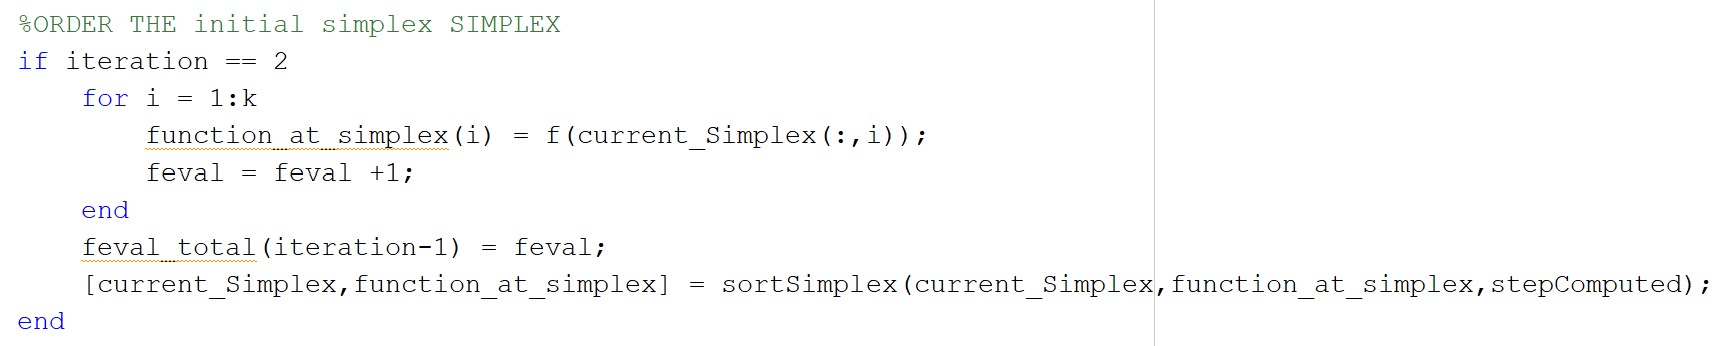
\includegraphics[width=0.95\linewidth]{Order1}
		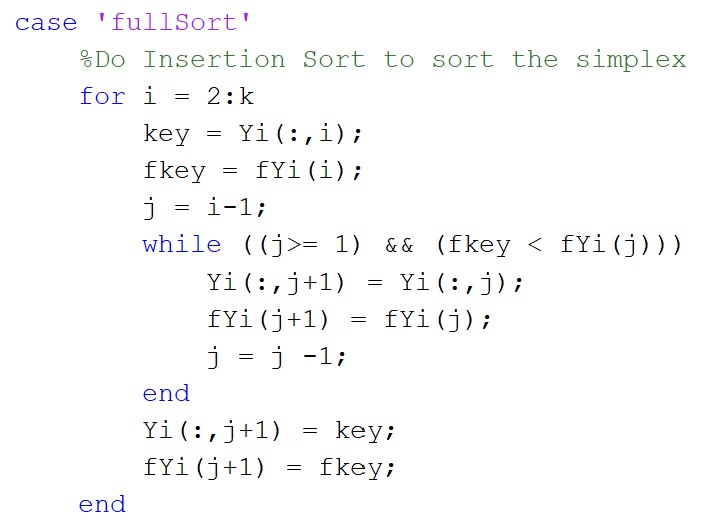
\includegraphics[width=0.95\linewidth]{Shrink2}
	\end{column}
	\begin{column}{0.59\linewidth}
		\centering
		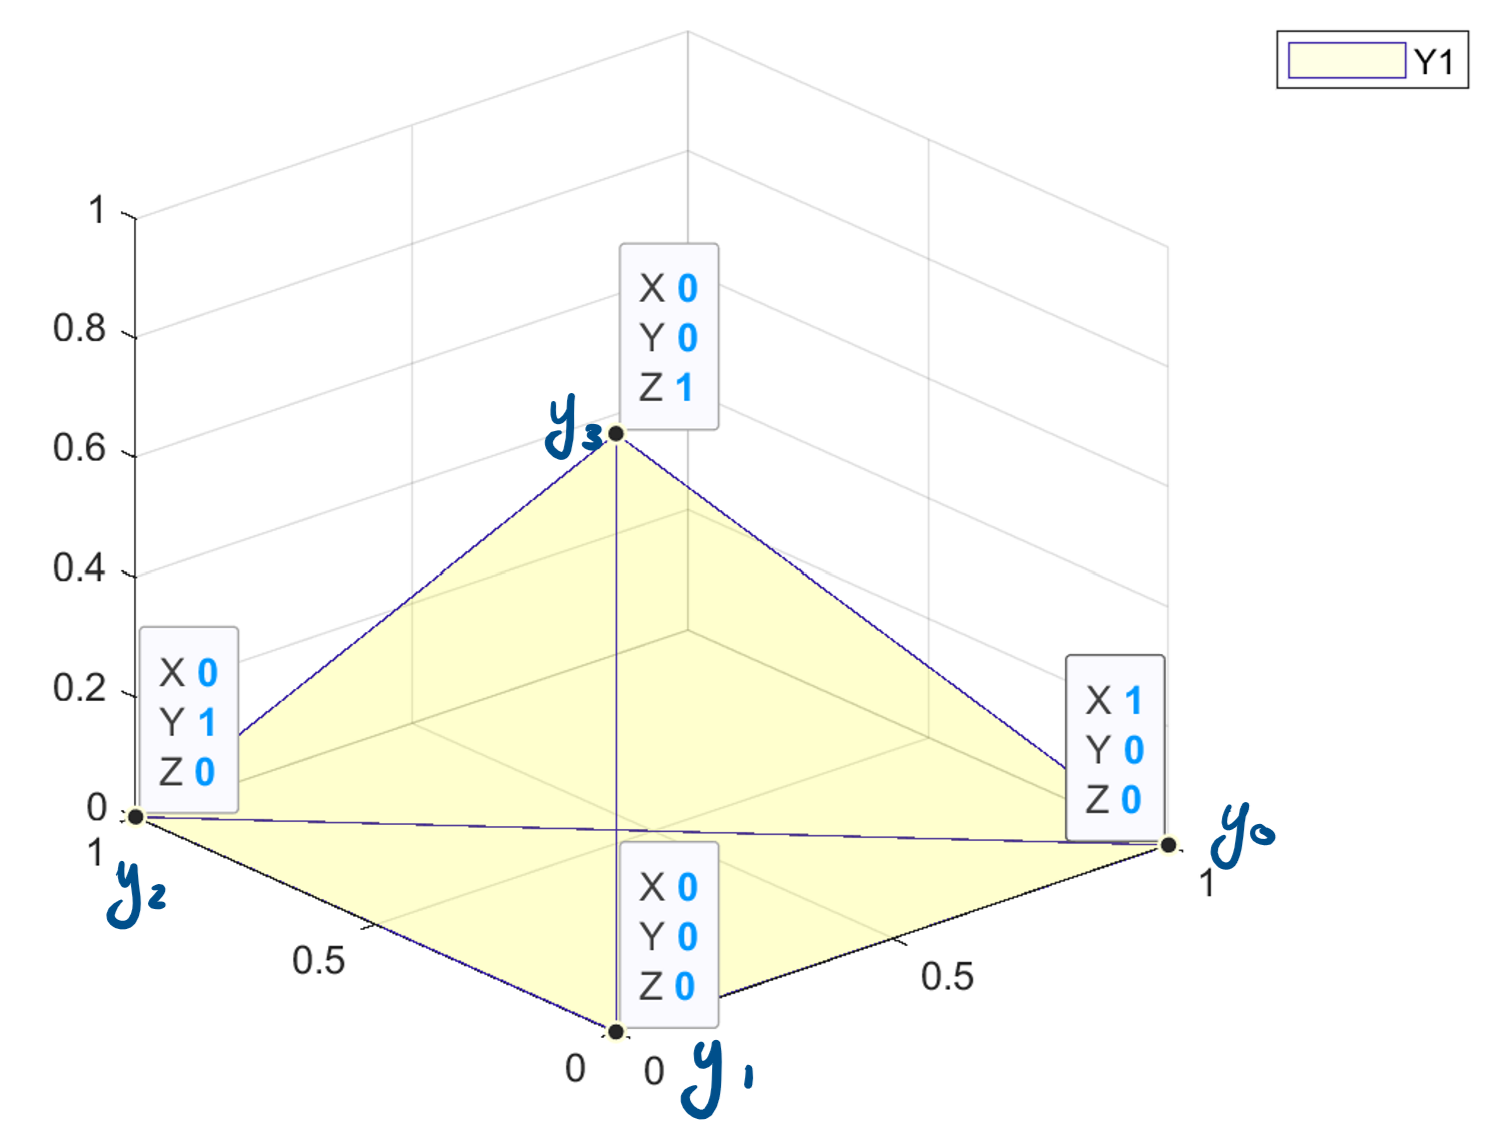
\includegraphics[width=0.95\linewidth]{Order1Fig}
	\end{column}
	\end{columns}
\end{frame}

\begin{frame}{1 and 2. Calculate centroid and $x^r$}
	\begin{columns}
	\begin{column}{0.35\linewidth}
		\centering
		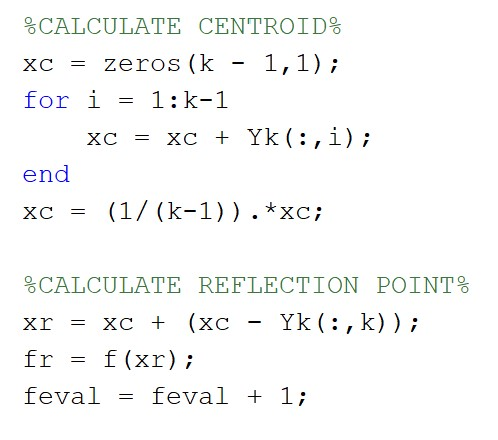
\includegraphics[width=0.95\linewidth]{Order2}
	\end{column}
	\begin{column}{0.59\linewidth}
		\centering
		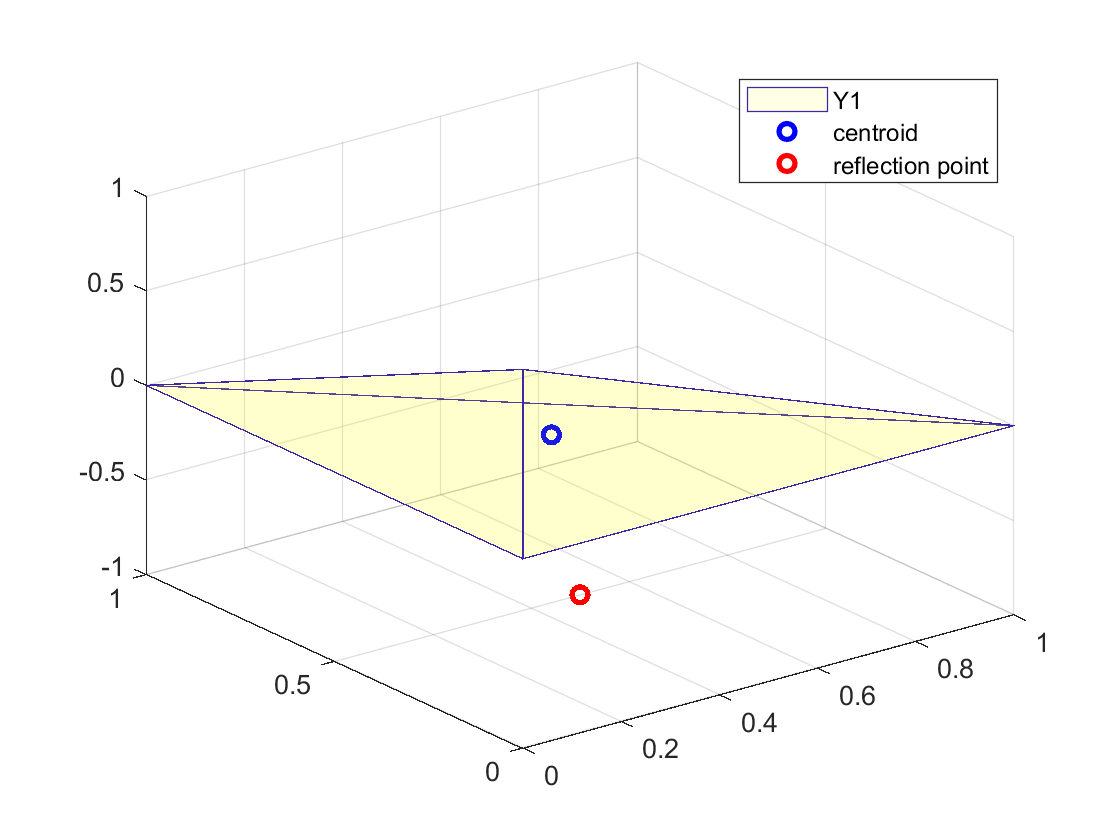
\includegraphics[width=0.95\linewidth]{Order2Fig}
	\end{column}
	\end{columns}
\end{frame}

\begin{frame}{2. Reflect}
	\begin{columns}
	\begin{column}{0.39\linewidth}
		\centering
		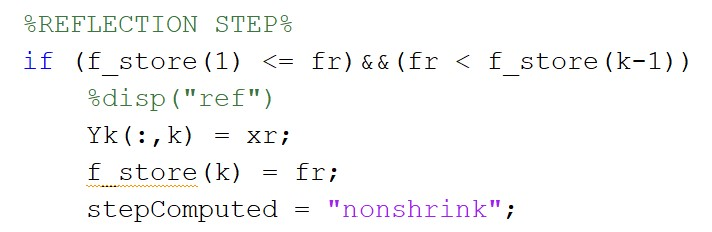
\includegraphics[width=0.95\linewidth]{Reflect}
	\end{column}
	\begin{column}{0.59\linewidth}
		\centering
		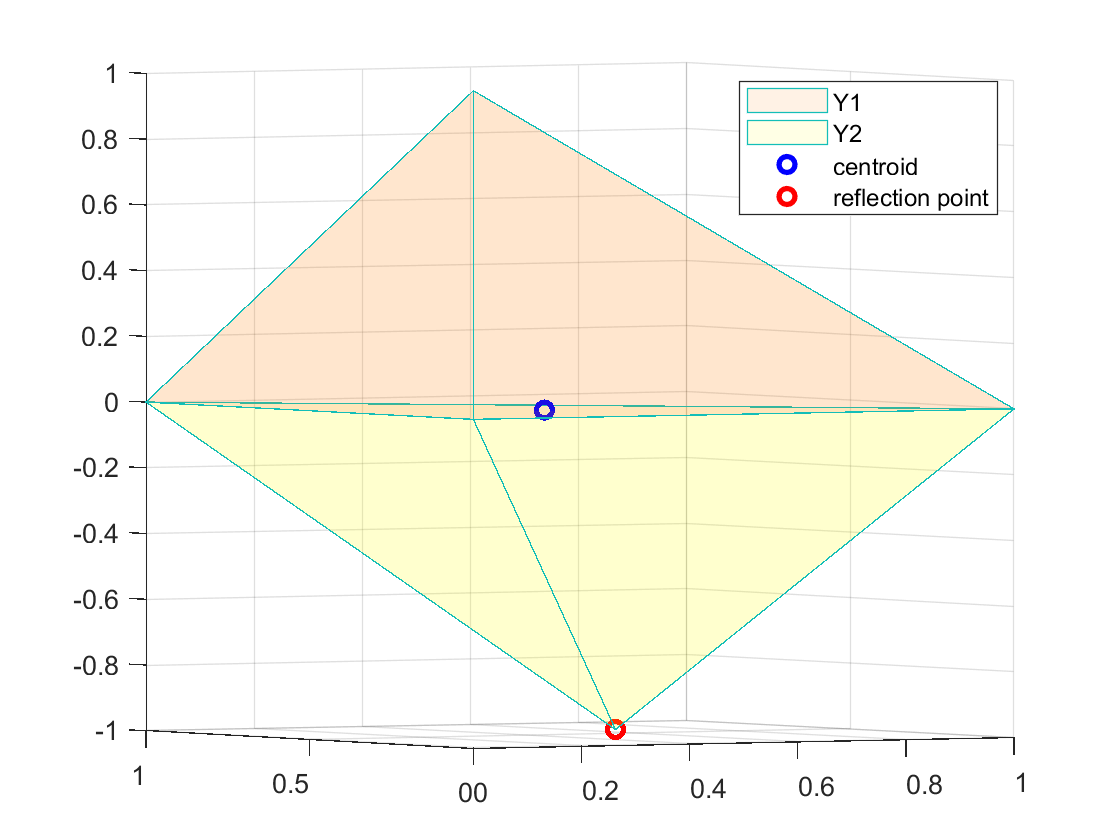
\includegraphics[width=0.95\linewidth]{ReflectFig}
	\end{column}
	\end{columns}
\end{frame}

\begin{frame}{3. Expand}
	\begin{columns}
	\begin{column}{0.39\linewidth}
		\centering
		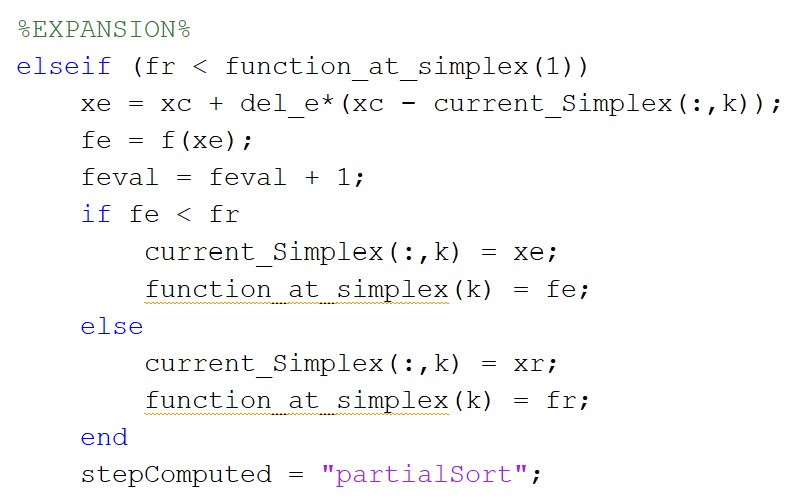
\includegraphics[width=0.95\linewidth]{Expand}
	\end{column}
	\begin{column}{0.59\linewidth}
		\centering
		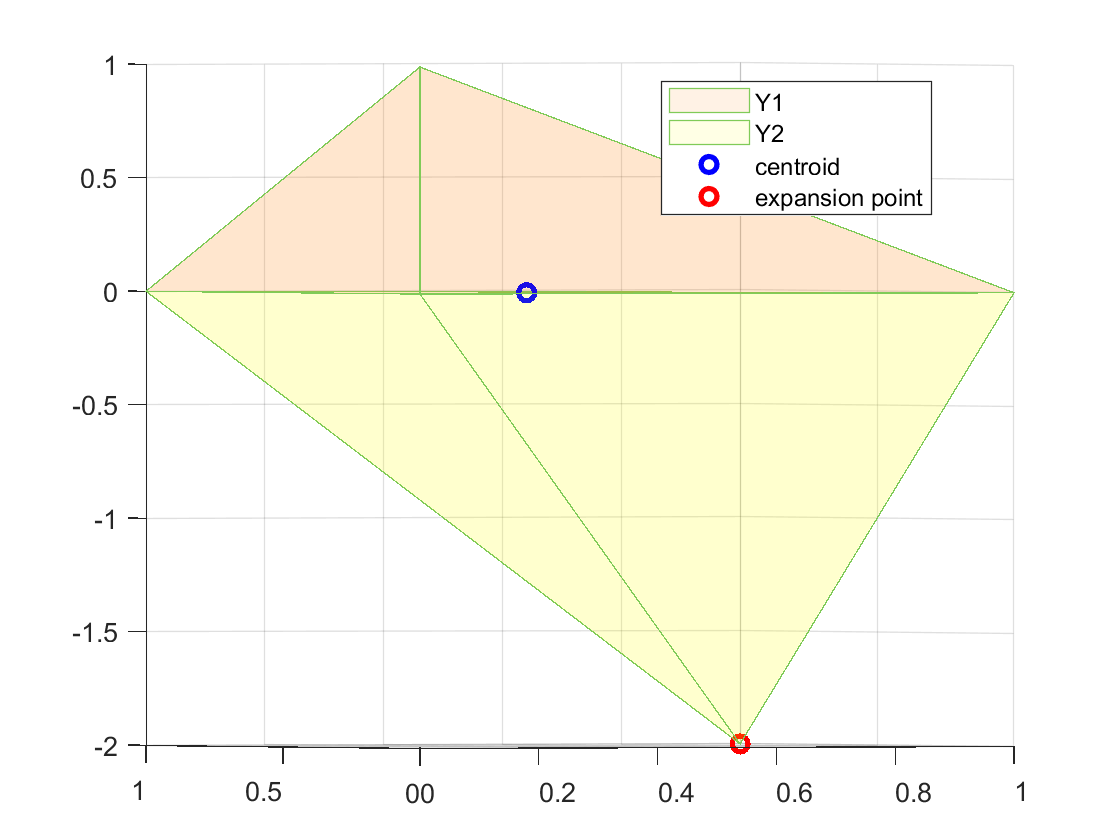
\includegraphics[width=0.95\linewidth]{ExpandFig}
	\end{column}
	\end{columns}
\end{frame}

\begin{frame}{4.a) Outside Contraction}
	\begin{columns}
	\begin{column}{0.39\linewidth}
		\centering
		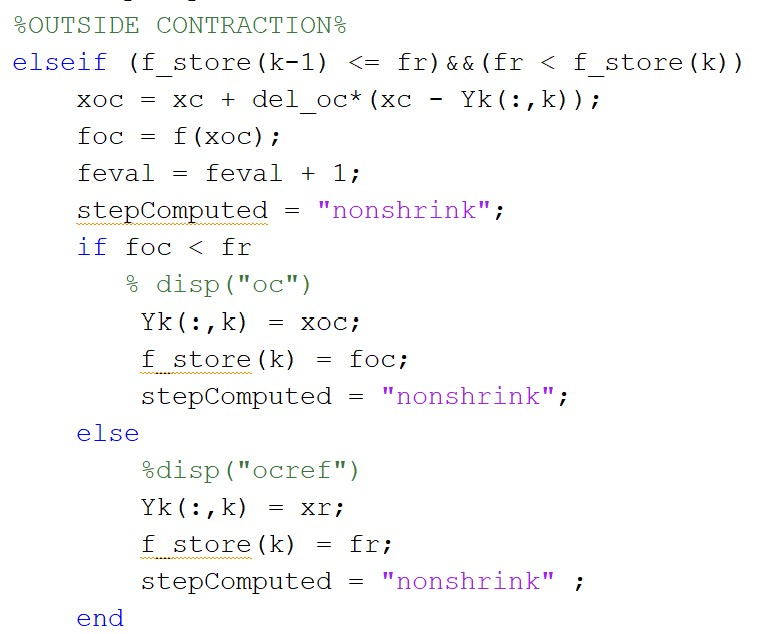
\includegraphics[width=0.95\linewidth]{OC}
	\end{column}
	\begin{column}{0.59\linewidth}
		\centering
		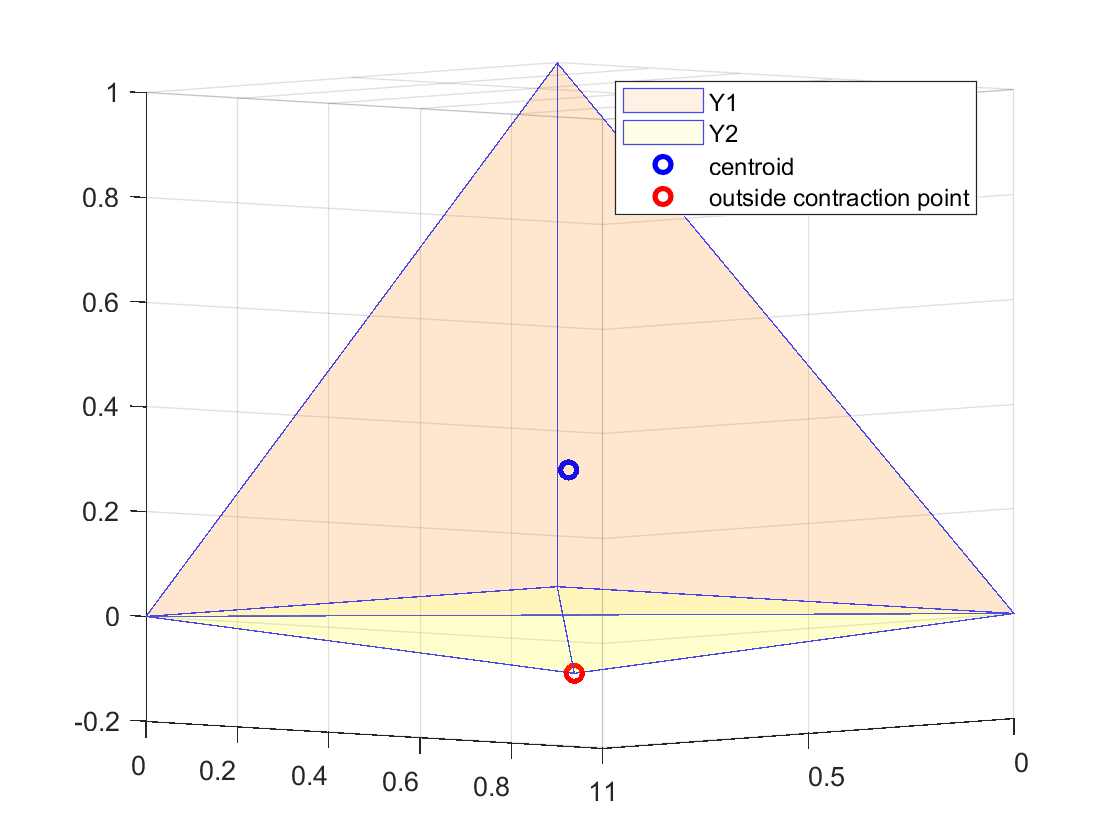
\includegraphics[width=0.95\linewidth]{OCFig}
	\end{column}
	\end{columns}
\end{frame}

\begin{frame}{4.b) Inside Contraction}
	\begin{columns}
	\begin{column}{0.39\linewidth}
		\centering
		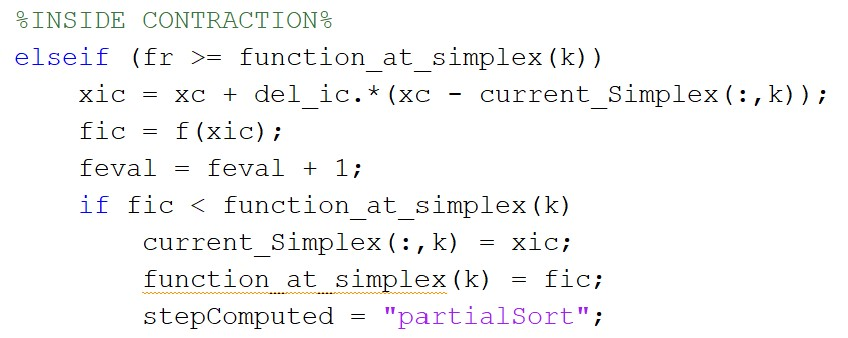
\includegraphics[width=0.95\linewidth]{IC}
	\end{column}
	\begin{column}{0.59\linewidth}
		\centering
		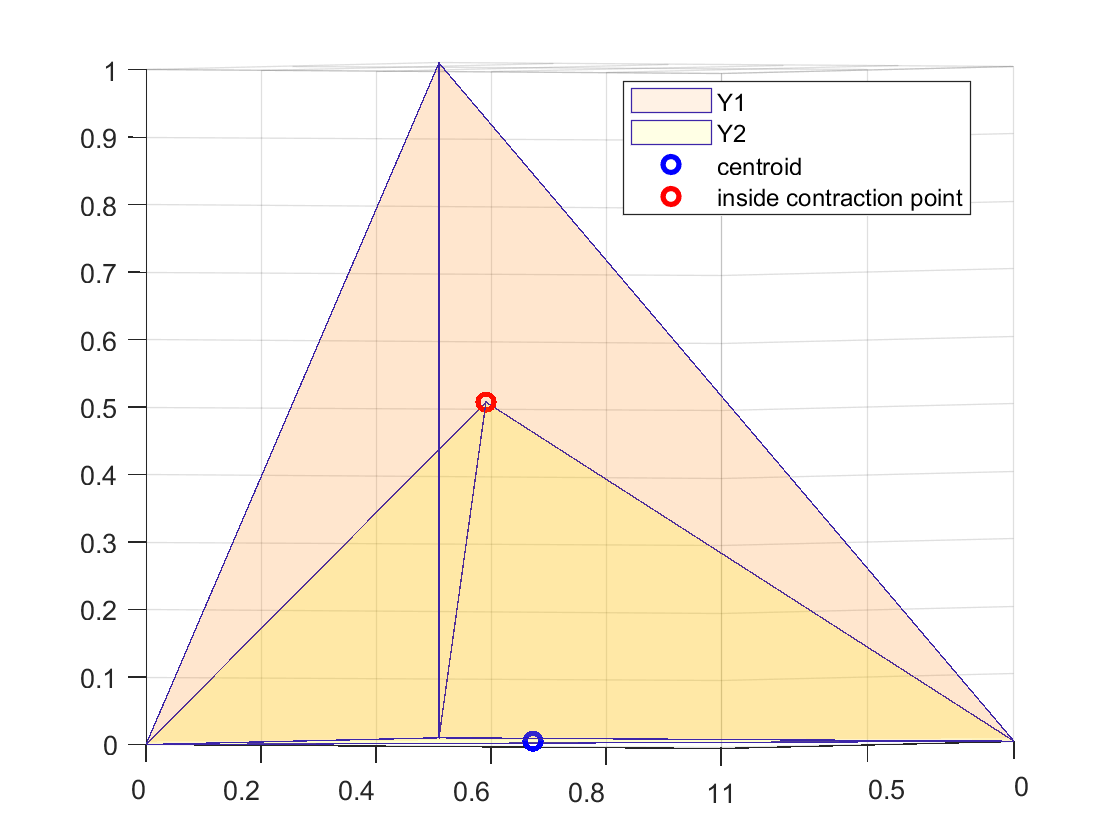
\includegraphics[width=0.95\linewidth]{ICFig}
	\end{column}
	\end{columns}
\end{frame}

\begin{frame}{5. Shrink}
	\begin{columns}
	\begin{column}{0.39\linewidth}
		\centering
		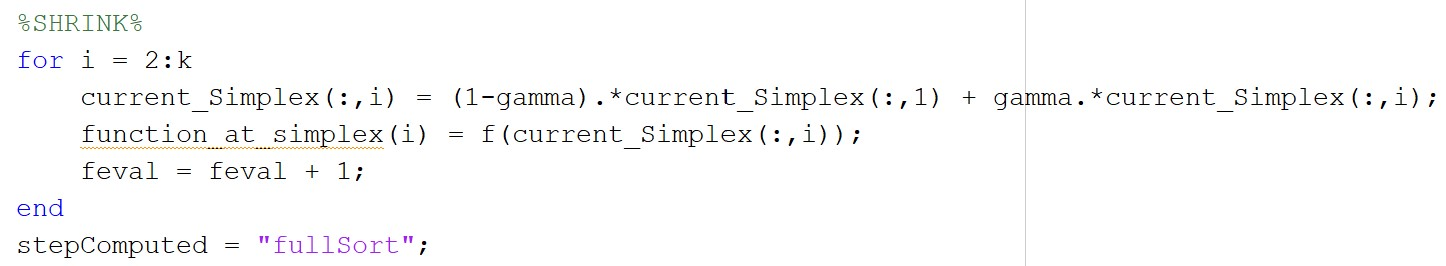
\includegraphics[width=0.95\linewidth]{Shrink}
		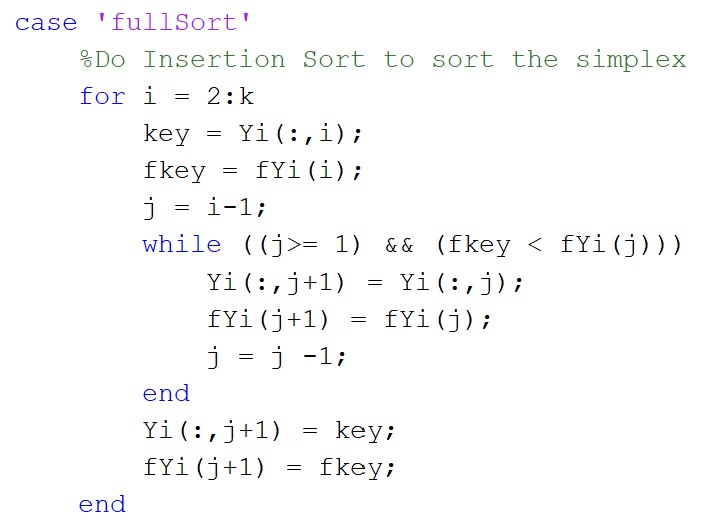
\includegraphics[width=0.85\linewidth]{Shrink2}
	\end{column}
	\begin{column}{0.59\linewidth}
		\centering
		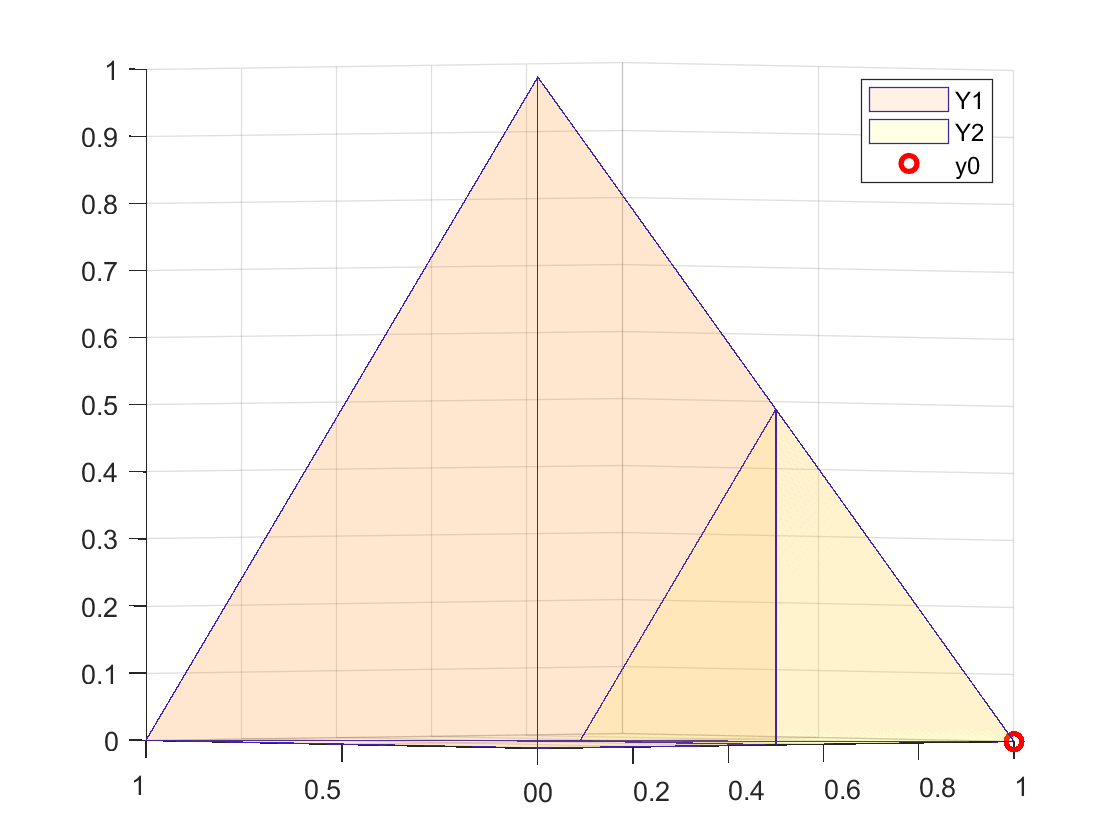
\includegraphics[width=0.95\linewidth]{ShrinkFig}
	\end{column}
	\end{columns}
\end{frame}

%%%%Examples
%------------------------------------------------------------------------
\begin{frame}{Examples of Nelder-Mead at work: A nice example}
\begin{columns}
\begin{column}{0.4\linewidth}
	plot of a nice function goes here	
\end{column}
\begin{column}{0.58\linewidth}
	put a convergence plot here and the min that we observe vs what our NM code takes us to
\end{column}
\end{columns}
\end{frame}

\begin{frame}{Examples of Nelder-Mead at work: Rosenbrock function}
\begin{columns}
\begin{column}{0.4\linewidth}
	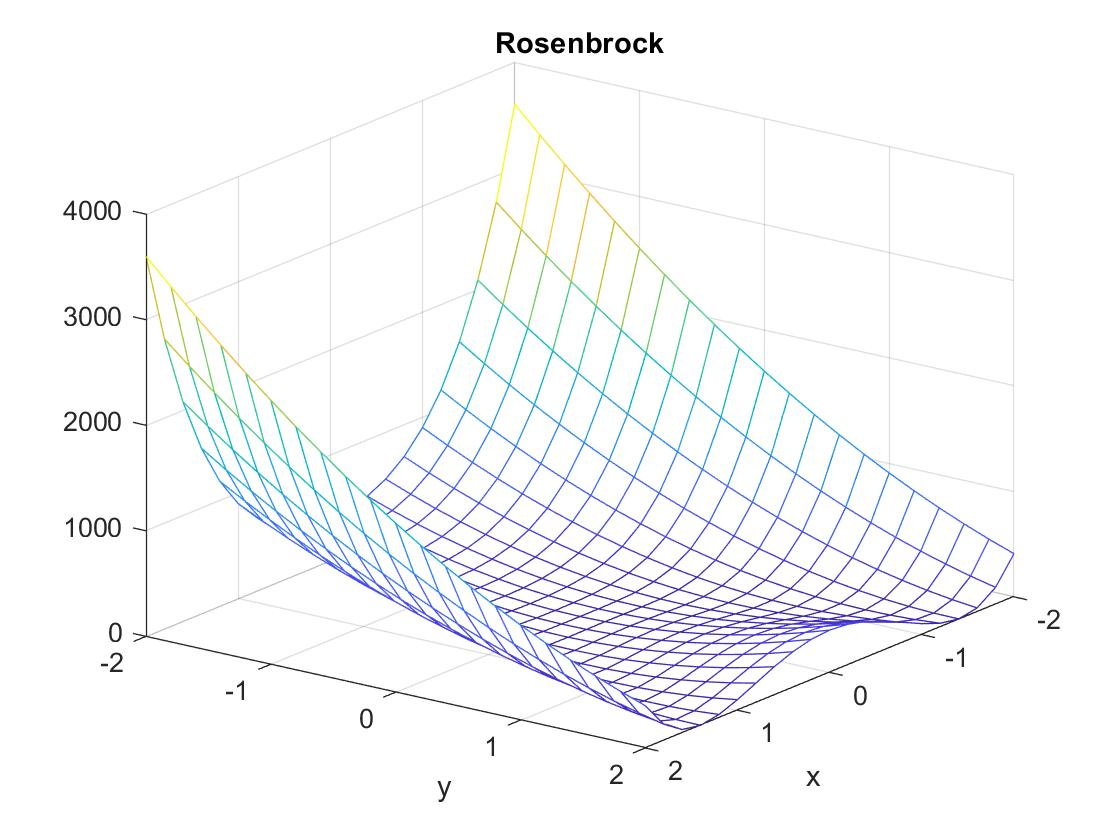
\includegraphics[width=0.95\linewidth]{rosenbrockPlotS1}
\end{column}
\begin{column}{0.58\linewidth}
	put a convergence plot here and the min that we observe vs what our NM code takes us to
\end{column}
\end{columns}
\end{frame}

\begin{frame}{Examples of Nelder-Mead at work: Rastrigin function}
\begin{columns}
\begin{column}{0.4\linewidth}
	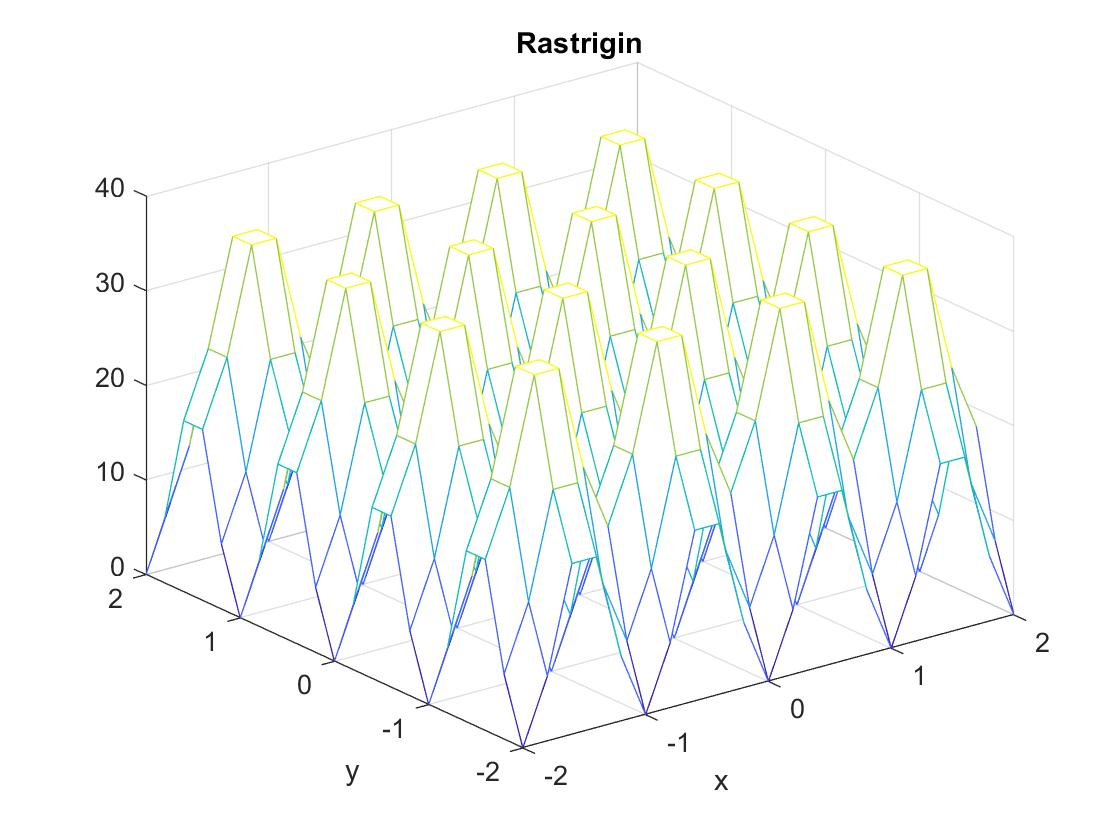
\includegraphics[width=0.95\linewidth]{rastriginPlotS1}	
\end{column}
\begin{column}{0.58\linewidth}
	put a convergence plot here and the min that we observe vs what our NM code takes us to
\end{column}
\end{columns}
\end{frame}


%%%%Solve the Rheology Problem
%------------------------------------------------------------------------
\begin{frame}{The Rheology Problem: Revisited}
%maybe turn this into 2 slides, one for standard and one for new params
	\begin{columns}
	\begin{column}{0.49\linewidth}
	\begin{block}{1. Standard parameters}
		Here is the code we gave to NM to run the standard parameters\\
		Here is the simplex and function values we obtained by running NM on the standard parameters
	\end{block}
	\end{column}
	\begin{column}{0.49\linewidth}
	\begin{block}{2. New parameters}
		We proposed new parameters using grid search on the parameter space\\
		Here is the code we gave to NM to run the new parameters\\
		Here is the simplex and function values we obtained by running NM on our new parameters
	\end{block}
	\end{column}
	\end{columns}
\end{frame}

\begin{frame}{The Rheology Problem: Revisited}
	\begin{columns}
	\begin{column}{0.39\linewidth}
		\centering
		Here is our convergence plot code
	\end{column}
	\begin{column}{0.59\linewidth}
		\centering
		Here is our convergence plot of all the cases
	\end{column}
	\end{columns}
\end{frame}


\end{document}